Before we progress with the study of Type Ia SNe found in the survey,
we take a detour to discuss an very interesting transient that turned
out not to be a SN~Ia. The transient, designated either SN SCP06F6 or
SCP 06F6, was first detected in February 2006. It was originally
reported in a June 2006 IAU circular \citep{dawson06a} while detailed
data and a discussion were presented later in \citet{barbary09a}. Its
light curve rise-time of $\sim$100 days is inconsistent with all known
SN types, and its spectroscopic attributes are not readily matched to
any known variable. It is surprising to discover such a rare object in
a survey with \emph{HST}, given its extremely small field of view
relative to ground-based SN surveys. However, current indication are
that this is indeed what happened, as a few candidates bearing some
similarities have since been identified in vastly wider-area surveys.

%Supernova (SN) surveys are designed to detect the brightening of
%supernovae over timescales of days to weeks. They often cover large
%areas at high sensitivity. As a result, they are able to discover
%unusual and rare transients with similar timescales.  For example, in
%2006 the Lick Observatory Supernova Search (LOSS) discovered an
%optical transient in the galaxy M85 \citep{kulkarni07a,rau07b,ofek08a}
%with a light curve plateau of $\sim$80 days.  It is suggested that the
%origin of this transient is a stellar merger and that an entire class
%of similar transients, \emph{luminous red novae}, exists.  Other
%recent discoveries of rare objects include a Type Ia SN with a
%super-Chandrasekhar mass progenitor \citep{howell06a} from the
%Supernova Legacy Survey (SNLS) and SN 2005ap, the most luminous SN
%ever observed \citep{quimby07a} from the Texas Supernova Search
%(TSS).

We present photometry in \S\ref{sec:f6_phot} and spectroscopy in
\S\ref{sec:f6_spec}. In \S\ref{sec:f6_discussion}, we discuss
constraints on possible identities. 


\section{Photometry} \label{sec:f6_phot}

The transient was discovered on 21 February 2006 (UT) in a field
centered on cluster CL 1432.5+3332.8 (F; $z = 1.112$). This field was
imaged over nine epochs with a period of roughly three weeks.  The
 discovery occurred in the fourth epoch at a position $\alpha =
14^\mathrm{h} 32^\mathrm{m} 27^\mathrm{s}.40$, $\delta = +33^\circ 32'
24''.8$ (J2000.0).  The angular separation from the cluster center is
$35''$, corresponding to a projected physical separation at the
cluster redshift of 290 kpc.  Table~\ref{tab:lightcurve} gives a
summary of photometric observations.

There is no prior detection of a source at the transient's location in
the NRAO VLA Sky Survey \citep{condon98a} at 1.4~GHz to the survey
$5\sigma$ detection limit of 2.5~mJy beam$^{-1}$.  There is no X-ray
detection at this location in a 5 ks exposure in the Chandra Telescope
XBootes survey \citep{kenter05a} to the detection limit of $7.8 \times
10^{-15}~\mathrm{erg}~ \mathrm{cm}^{-2}~\mathrm{s}^{-1}$ in the full
0.5-7 keV band.

%%%%%%%%%%%%%%%%%%%%%%%%%%%%%%%%%%%%%%%%%%%%%%%%%%%%%%%%%%%%%%%%%%
% PHOTOMETRY TABLE                                               %
%%%%%%%%%%%%%%%%%%%%%%%%%%%%%%%%%%%%%%%%%%%%%%%%%%%%%%%%%%%%%%%%%%
\begin{table}[tbh]
\begin{center}
\caption{Photometric observations of SN SCP06F6\label{tab:lightcurve}}
\vspace{10pt}
\begin{footnotesizetabular}{l c c c c c c c}
\hline
\hline
     &       &     & Tele- &        & Exp. &             &           \\
Num. &  Date & MJD & scope & Filter & (s)  & Scaled Flux & Magnitude \\
\hline
1  & 11/28/05 & 53716.1 & \emph{HST} & $i_{775}$ & $175$  & $\phantom{-}0.0018 \pm 0.0049$  & $> 26.515$ \\
   &          &         &            & $z_{850}$ & $1400$ & $-0.0019 \pm 0.0053$            & $> 27.222$ \\
2  & 01/03/06 & 53738.7 & \emph{HST} & $i_{775}$ & $375$  & $\phantom{-}0.0002 \pm 0.0025$  & $> 27.509$ \\
   &          &         &            & $z_{850}$ & $1500$ & $\phantom{-}0.0053 \pm 0.0049$  & $26.733 \pm  0.857$ \\
3  & 01/29/06 & 53764.6 & \emph{HST} & $z_{850}$ & $1500$ & $\phantom{-}0.0087 \pm 0.0050$  & $26.185 \pm  0.524$ \\
4  & 02/21/06 & 53787.2 & \emph{HST} & $i_{775}$ & $515$  & $\phantom{-}0.1183 \pm 0.0032$  & $23.395 \pm  0.025$ \\
   &          &         &            & $z_{850}$ & $1360$ & $\phantom{-}0.1367 \pm 0.0059$  & $23.201 \pm  0.040$ \\
5  & 03/19/06 & 53813.7 & \emph{HST} & $i_{775}$ & $440$  & $\phantom{-}0.4229 \pm 0.0055$  & $22.012 \pm  0.012$ \\
   &          &         &            & $z_{850}$ & $1360$ & $\phantom{-}0.3805 \pm 0.0067$  & $22.089 \pm  0.016$ \\
6  & 04/04/06 & 53829.6 & \emph{HST} & $i_{775}$ & $515$  & $\phantom{-}0.6216 \pm 0.0065$  & $21.593 \pm  0.010$ \\
   &          &         &            & $z_{850}$ & $1360$ & $\phantom{-}0.6055 \pm 0.0074$  & $21.585 \pm  0.011$ \\
7  & 04/22/06 & 53847.0 & \emph{HST} & $i_{775}$ & $515$  & $\phantom{-}0.8343 \pm 0.0068$  & $21.274 \pm  0.008$ \\
   &          &         &            & $z_{850}$ & $1360$ & $\phantom{-}0.8276 \pm 0.0080$  & $21.246 \pm  0.009$ \\
8  & 05/21/06 & 53876.8 & \emph{HST} & $i_{775}$ & $295$  & $\phantom{-}1.0000 \pm 0.0099$  & $21.077 \pm  0.009$ \\
   &          &         &            & $z_{850}$ & $1400$ & $\phantom{-}1.0000 \pm 0.0082$  & $21.040 \pm  0.008$ \\
9  & 06/03/06 & 53889.3 & \emph{HST} & $i_{775}$ & $800$  & $\phantom{-}0.8534 \pm 0.0056$  & $21.249 \pm  0.006$ \\
   &          &         &            & $z_{850}$ & $1200$ & $\phantom{-}0.9176 \pm 0.0081$  & $21.134 \pm  0.008$ \\
10 & 06/28/06 & 53914.4 & Subaru     & $i_{775}$ & $960$  & $\phantom{-}0.6290 \pm 0.1441$  & $21.581 \pm  0.211$ \\
   &          &         &            & $z_{850}$ & $480$  & $\phantom{-}0.7384 \pm 0.1520$  & $21.370 \pm  0.189$ \\
11 & 08/23/06 & 53970.3 & Subaru     & $i_{775}$ & $600$  & $\phantom{-}0.0586 \pm 0.0234$  & $24.158 \pm  0.368$ \\
   &          &         &            & $z_{850}$ & $600$  & $\phantom{-}0.0654 \pm 0.0875$  & $> 23.080$ \\
12 & 05/18/07 & 54238.5 & Subaru     & $i_{775}$ & $2280$ & $-0.0324 \pm 0.0201$            & \ldots \\
\hline
\end{footnotesizetabular}

\end{center}
{\footnotesize
{\bf Note.} --- Flux measurements scaled relative to highest flux
epoch; effective zeropoints are 21.077 for $i_{775}$ and 21.040 for
$z_{850}$.
}
\end{table}

%%%%%%%%%%%%%%%%%%%%%%%%%%%%%%%%%%%%%%%%%%%%%%%%%%%%%%%%%%%%%%%%%%
% IMAGE                                                          %
%%%%%%%%%%%%%%%%%%%%%%%%%%%%%%%%%%%%%%%%%%%%%%%%%%%%%%%%%%%%%%%%%%
\begin{figure}
\begin{center}
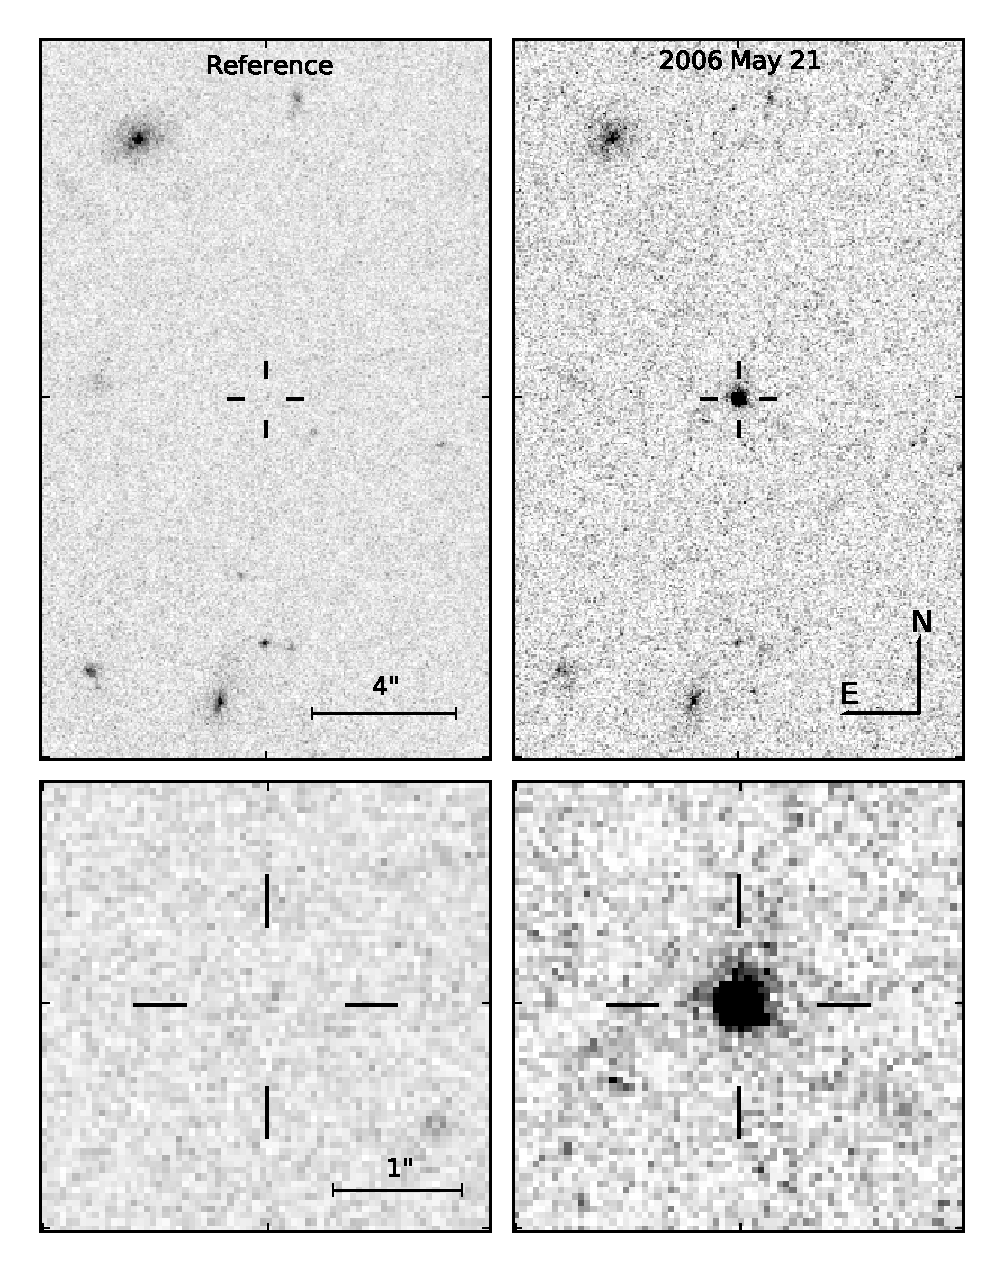
\includegraphics[width=0.9\textwidth]{figures/scp06f6/images.eps}
\end{center}
\caption[Imaging of SN SCP06F6]{Deep stack of the first three epochs
  in $z_{850}$ totaling 4400~s where the transient is undetected
  (\emph{top left} and zoomed in, \emph{bottom left}), and the
  highest-flux epoch eight $z_{850}$ exposure of 1400~s (\emph{top
    right} and zoomed in, \emph{bottom right}).  All images have the
  same greyscale.  The hash marks indicate the transient position and
  have the same physical scale in all images.\label{fig:images}}
\end{figure}

%%%%%%%%%%%%%%%%%%%%%%%%%%%%%%%%%%%%%%%%%%%%%%%%%%%%%%%%%%%%%%%%%%
% LIGHTCURVE PLOT                                                %
%%%%%%%%%%%%%%%%%%%%%%%%%%%%%%%%%%%%%%%%%%%%%%%%%%%%%%%%%%%%%%%%%%
\begin{figure}
\begin{center}
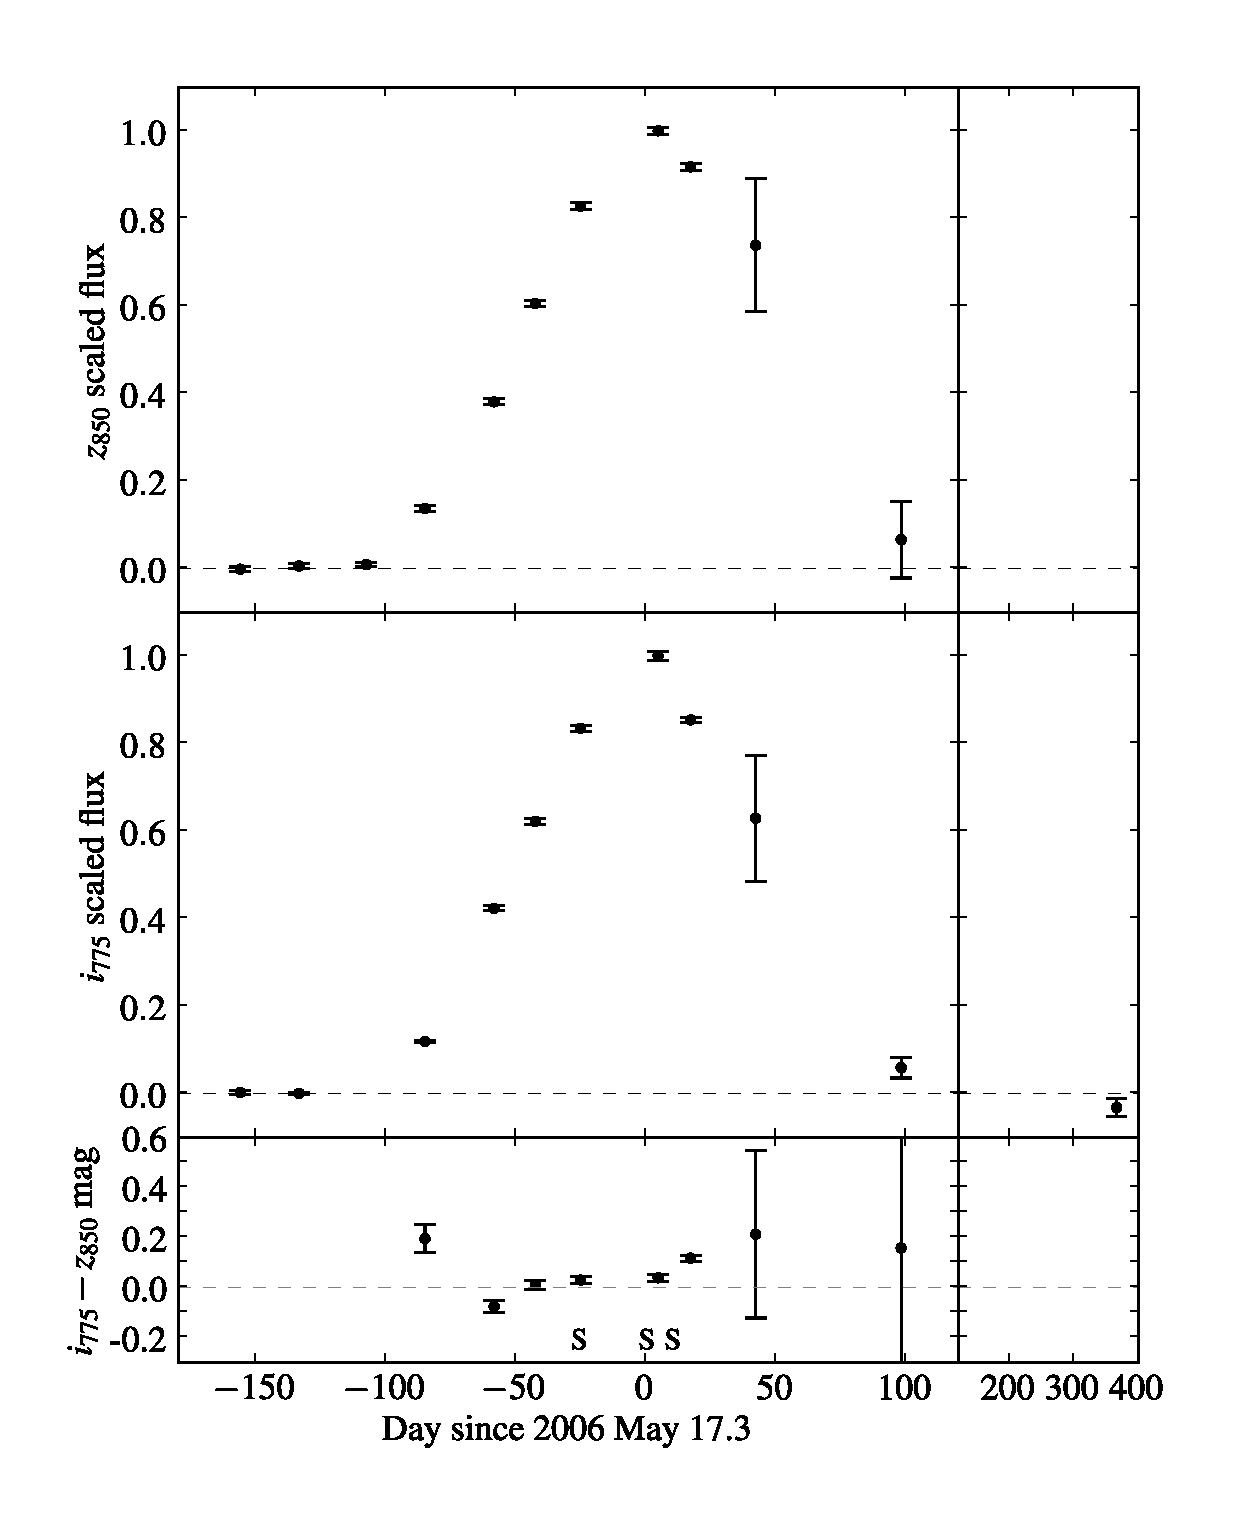
\includegraphics[width=0.9\textwidth]{figures/scp06f6/lightcurve.eps}
\end{center}
\caption[Light curve of SN SCP06F6]{Flux light curve for $z_{850}$
  (\emph{top panel}) and $i_{775}$ (\emph{middle panel}) scaled to
  maximum flux.  The last three epochs (starting at +42 days) are
  Subaru FOCAS observations.  \emph{bottom panel}: $i_{775} - z_{850}$
  color for epochs with significant detection in both bands. Though
  the color only varies $\sim 0.2$ magnitudes between the five best
  measured epochs, there is evidence for evolution.  The spectral
  epochs are marked along the abscissa with an ``S.''
	 \label{fig:lightcurve}}
\end{figure}

The transient is consistent with a point source in each of the six ACS 
detection epochs to the extent we can determine.
We performed aperture photometry on the {\sc MultiDrizzle}-processed ACS images
using 3.0 pixel ($0''.15$) radius apertures for $i_{775}$ and 5.0~pixel 
($0''.25$) radius apertures for $z_{850}$. Aperture corrections were taken 
from Table~3 of \citet{sirianni05a}. The systematic error due to the known 
color dependence of $z_{850}$ aperture correction \citep[see][]{sirianni05a} 
is estimated to be less than 0.015~mag.

After the transient had left the visibility window of \emph{HST} it remained 
visible from Mauna Kea for several months. Three additional photometry points 
were obtained with the Faint Object Camera and Spectrograph 
\citep[FOCAS;][]{kashikawa02a} 
on the Subaru telescope on 2006 June 28, 2006 August 23, 
and the next year on 2007 May 18. The June observations suffered from poor 
weather conditions (seeing $\gtrsim 2''$). 
All observations were cosmic ray-rejected using 120~s exposures. 
We performed aperture photometry using a $1''.04$ radius aperture and 
estimated photometric errors as described by \citet{morokuma08a}. 
In order to express magnitudes in the ACS filter 
system, we determined Subaru image zeropoints by cross-correlating the 
photometry of nine surrounding stars in the ACS and Subaru images. The 
Subaru FOCAS $i'$ and $z'$ filters are similar enough to ACS $i_{775}$ and 
$z_{850}$ that there is no significant trend with stellar color.

A deep stack of the first three epochs in $z_{850}$ totaling 4400~s 
(Fig.~\ref{fig:images}) and first two epochs 
in $i_{775}$ totaling 550~s provide limits on the magnitude of a possible 
progenitor star (if galactic) or host galaxy (if extragalactic).
No progenitor star is detected in a 3.0~pixel radius aperture centered at the 
position of the transient (known to $< 0.2$~pixels) to a $3\sigma$ upper limit 
of $i_{775} > 26.4$ and $z_{850} > 26.1$ 
(Vega magnitudes are used throughout this Letter).
There is no sign of a host galaxy in the 1~arcsec$^2$ surrounding the 
transient to a surface brightness $3\sigma$ limit of 25.0~mag~arcsec$^{-2}$ and 
25.1~mag~arcsec$^{-2}$ in $z_{850}$ and $i_{775}$, respectively.
However, there is a $6\sigma$ detection in a 3.0~pixel radius aperture of a 
$\sim$25.8~mag object $1''.5$ southwest of the 
transient position in $z_{850}$ (Fig.~\ref{fig:images}, \emph{lower left}). 
If the transient is extragalactic, this might represent a faint host galaxy.

The transient increased in brightness in each of 
epochs four through eight before finally declining in the ninth epoch, 
resulting in a rise time of approximately 100~days 
(Fig. \ref{fig:lightcurve}). 
A fit to the brightest five ACS $z_{850}$ photometry points 
gives a date of max of 2006 May 17.3 (MJD 53872.3). 
The declining part of the light curve, although sparsely measured, 
is consistent with symmetry about the maximum. 
The final photometry point approximately one year after maximum light shows 
no detection. The $i_{775} - z_{850}$ color is approximately constant over 
the 50~days preceding maximum light, but does show significant signs of 
evolution at early times and after maximum light.


\section{Spectroscopy} \label{sec:f6_spec}

%%%%%%%%%%%%%%%%%%%%%%%%%%%%%%%%%%%%%%%%%%%%%%%%%%%%%%%%%%%%%%%%%%
% SPECTROSCOPY PLOT                                              %
%%%%%%%%%%%%%%%%%%%%%%%%%%%%%%%%%%%%%%%%%%%%%%%%%%%%%%%%%%%%%%%%%%
\begin{figure}
\begin{center}
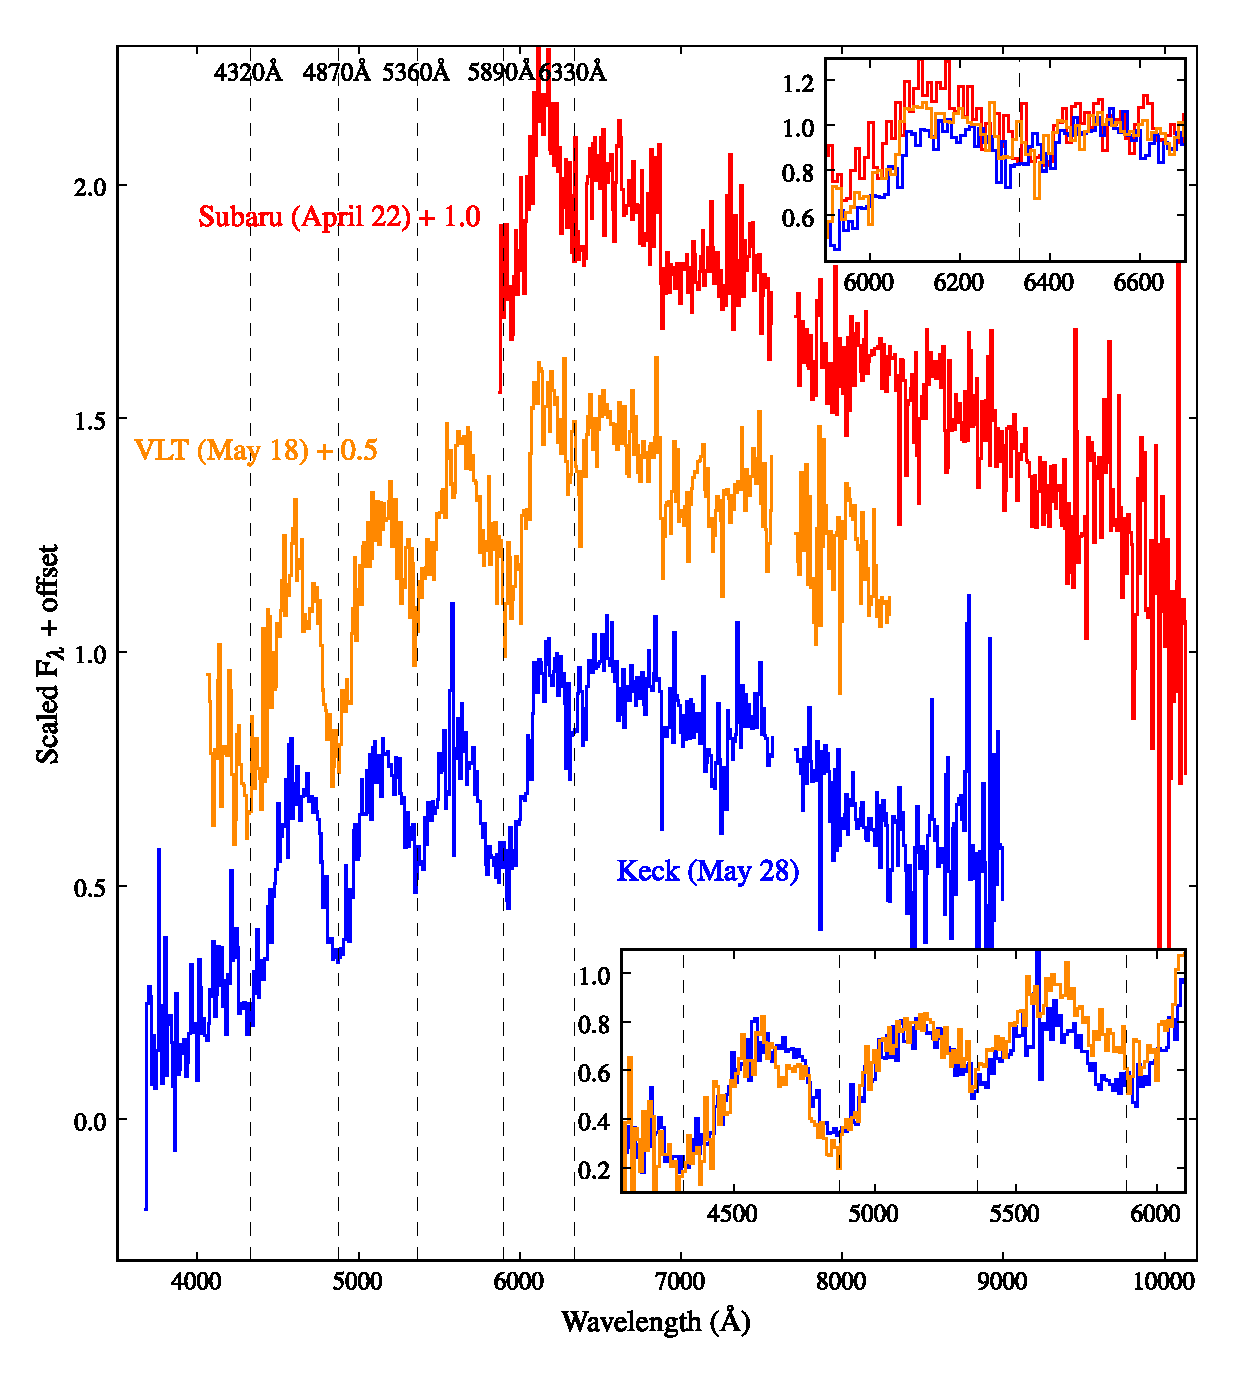
\includegraphics[width=\textwidth]{figures/scp06f6/spectra.eps}
\end{center}
\caption[Spectroscopy of SN SCP06F6]{Spectra averaged in
  10~\AA\ bins. Vertical dotted lines indicate the approximate
  absorption band centroids. Spectra are normalized to match in the
  red continuum. Inset figures show regions where spectra differ.
  \emph{Top Inset}: Overplot of all three spectra in the range
  5900~\AA\ - 6700~\AA, demonstrating apparent evolution of the flux
  at $\sim$6150~\AA\ relative to the red continuum.  \emph{Bottom
    Inset}: Overplot of VLT and Keck spectra (no offset) demonstrating
  apparent evolution at 4670~\AA\ and of the absorption feature at
  5890~\AA.\label{fig:spectra}}
\end{figure}

Spectroscopy was acquired on three dates (Fig.~\ref{fig:spectra}): 
2006 April 22 (-25~days) using Subaru FOCAS, 
2006 May 18 (+1~day) using VLT FORS2 \citep{appenzeller98a}, and 
2006 May 28 (+11~days) with Keck LRIS \citep{oke95a}.
The Subaru spectrum covers wavelengths longward of 5900~\AA, 
while the VLT and Keck spectra cover bluer wavelengths.
The VLT spectrum (observed at airmass $> 2$) is corrected for differential 
slit loss by applying a linear correction with a slope of 0.25 per 1000~\AA, 
derived from a comparison to the Keck spectrum, which covers the 
entire wavelength range of the VLT spectrum.
The Keck observation was made at the parallactic angle, 
while Subaru FOCAS is equipped with an atmospheric dispersion corrector,
making these observations more reliable measures of relative flux.

The spectra show a red continuum and several broad absorption features: 
a possible absorption feature at 4320~\AA\ ($\mathrm{FWHM} \sim 180$~\AA), 
three strong features at 4870~\AA\ ($\mathrm{FWHM} \sim 200$~\AA), 
5360~\AA\ ($\mathrm{FWHM} \sim 230$~\AA) and 5890~\AA\ 
($\mathrm{FWHM} \sim 280$~\AA), 
and a weaker absorption feature at 6330~\AA\ ($\mathrm{FWHM} \sim 270$~\AA). 
Including uncertainty in continuum shape, errors are estimated to be 25~\AA.

We compared the spectra to all supernova types using the $\chi^2$ fitting 
program described in \citet{howell05a} as well as the program SNID 
\citep{blondin07a}. No match was found with either program.

If the transient is galactic ($z=0$),
the absorption features at 4320~\AA\ and 4870~\AA\ are consistent with
$\mathrm{H}\gamma$ (4341~\AA) and $\mathrm{H}\beta$ (4861~\AA) respectively.
However, there is no significant $\mathrm{H}\alpha$ (6563~\AA) emission or 
absorption, which would be expected for the presence of strong 
$\mathrm{H}\gamma$ and $\mathrm{H}\beta$ features. (Although there is 
slight evidence for emission at 6563~\AA\ in the 
Keck spectrum, this is not seen in the VLT or Subaru spectra.)
It is therefore unlikely that the 4320~\AA\ and 4870~\AA\ features are 
due to hydrogen.
No other narrowband emission or absorption lines are detected.
From the slope of the red continuum we derive a lower limit blackbody 
temperature of 6500 K. The shape of the continuum is inconsistent with 
$\mathrm{F}_\lambda \propto \lambda^{-5/3}$ synchrotron radiation. 

If the transient is extragalactic, the absence of Lyman $\alpha$ absorption 
features shortward of 4500 \AA\ places a hard upper limit of $z \lesssim 2.7$ on 
its redshift. Among redshifts $0 < z < 2.7$, the cluster redshift of 
$z = 1.112$ is of specific interest;
the transient is located a small projected distance from the center of the 
cluster. At this redshift,
the absorption feature at 5890~\AA\ is consistent with Mg \textsc{ii}
$\lambda\lambda2796,2803$. However, the remaining features are not identified 
at this redshift. At $z = 1.112$, a peak apparent magnitude of 
$i_{775} = 21.0$ implies a peak bolometric magnitude of approximately $-22.1$.

A comparison of the three spectra shows evidence for spectral evolution.
The flux at 
$\sim$6150~\AA\ consistently decreases relative to the red continuum over time
(Fig.~\ref{fig:spectra}, \emph{upper inset}).
Over the 10 day period from the VLT to the Keck spectrum, 
the absorption feature at 5890~\AA\ appears to move toward shorter wavelengths,
while a small absorption feature at 4670~\AA\ in the VLT spectrum 
seems to disappear in the Keck spectrum
(Fig.~\ref{fig:spectra}, \emph{lower inset}).


\section{Discussion} \label{sec:f6_discussion}

The key features of SN SCP06F6 are as follows: a rise time of
$\sim$100~days with a roughly symmetric light curve; small but
statistically significant color variations across the light curve; no
detected host galaxy or progenitor; broad spectral features in the
blue, with a red continuum, and some evidence for spectral evolution.
Below, we first discuss constraints on the distance to the source.
Next we consider the possibility that the transient is the result of
microlensing, finding this to be unlikely.  Lastly, we search for
objects in the SDSS spectral database, finding no convincing matches.

%%%%%%%%%%%%%%%%%%%%%%%%%%%%%%%%%%%%%%%%%%%%%%%%%%%%%%%%%%%%%%%%%%%%
% PROPER MOTION PLOT                                               %
%%%%%%%%%%%%%%%%%%%%%%%%%%%%%%%%%%%%%%%%%%%%%%%%%%%%%%%%%%%%%%%%%%%%
\begin{figure}[tbh]
\begin{center}
\includegraphics[width=0.8\textwidth]{figures/scp06f6/propmotion.eps}
\end{center}
\caption[Proper motion of SN SCP06F6]{Position of the transient in
  each of the 6 ACS detection epochs.  1 pixel is $0''.05$. The upper
  limit on parallax is 0.3 pixels.\label{fig:propmotion}}
\end{figure}

\subsection{Distance from Parallax}
Any detection of proper motion or parallax would be strong evidence of
a galactic source. We tested for this by fitting the position of the
transient in each of the six ACS detection epochs using a
two-dimensional Gaussian (Fig.~\ref{fig:propmotion}).  The fit
uncertainty is dominated by residual distortion and alignment errors
in most epochs.  These errors are on the order of 0.1 to 0.2~pixels.
The most discrepant positions differ by approximately 0.25~pixels
($0''.0125$).  As a whole, the positions are consistent with no proper
motion or parallax and give little indication of either.  The upper
limit on parallax is 0.3~pixels ($0''.015$), which gives a lower limit
on distance of $\sim$70~pc.

\subsection{Distance from Reference Limits}
We can derive a more significant constraint on distance from reference
image magnitude limits, assuming that the transient is an explosion
and a progenitor star exists. The dimmest stars (aside from neutron
stars) known to undergo explosions are white dwarfs (WDs).  WDs range
in absolute magnitude from approximately 10~mag
($T_\mathrm{eff}\sim25000$~K) to approximately 16~mag
($T_\mathrm{eff}\sim3000$~K).  If we assume the progenitor is a WD
with absolute magnitude $i_{775} = 13$, the reference image $3\sigma$
upper limit of $i_{775} > 26.4$ gives a distance $3\sigma$ lower limit
of 4.8~kpc. Because the source is at high galactic latitude ($b =
67.3^\circ$), we are looking nearly directly out of the plane of the
galaxy. Given a Milky Way scale height for WDs of $(275 \pm 50)$~pc
\citep{boyle89a}, this places the source firmly outside of the plane
of the Galaxy. However, a galactic WD progenitor is still possible, if
it is a relatively cool white dwarf residing in the galactic halo. If
the progenitor is a source dimmer than $i_{775} = 13$~mag (e.g., a
cooler WD or neutron star), the constraints on distance are weaker.

\subsection{A Microlensing Event?}
Although the symmetry of the light curve (Fig.~\ref{fig:lightcurve})
suggests that the transient is a microlensing event, this
interpretation is unlikely.  The light curve is dramatically broader
than the theoretical light curve for microlensing of a point source by
a single lens \citep{paczynski86a}. The typical light curve FWHM of
high-magnification (peak magnification $\gtrsim 300$) microlensing
events is on the order of a few hours \citep[e.g.,][]{abe04a,dong06a}
whereas the transient's light curve FWHM is $\sim$100 days with a peak
magnification $3\sigma$ lower limit of $\sim$120.  Also, the color
evolves a small but significant amount over the light curve,
particularly between epochs eight and nine. Some of these difficulties
can be overcome if we assume the source is resolved; this can both
change the shape of the light curve and allow for color variation as
different source regions are differentially magnified. However, this
typically results in a lower peak magnification. Finally, microlensing
would still not explain the mysterious spectrum.

\subsection{Search for Similar Objects in SDSS}
In an effort to identify objects with similar spectra, we
cross-correlated the broad features of the spectrum with the SDSS
spectral database. Each SDSS spectrum was warped with a polynomial
function to best fit the Keck spectrum, based on a least squares
fit. The value of the root mean square of the difference between the
spectra was used to determine the correlation. An allowance for
relative redshift was made, with the requirement that the spectra
overlapped in the range of the strongest features (3500~\AA\ to
6200~\AA). No convincing matches were found. Changing the warping
function between linear and quadratic and varying the wavelength range
used in the fit altered which SDSS objects had the highest
correlation, but did not result in a more convincing match. The SDSS
objects with the highest correlation were broad absorption line
quasars (BAL QSOs) at various redshifts and carbon (DQ) WDs.  Although
BAL QSOs do have similarly broad features, they don't exhibit the
spacing or rounded profiles of those of the transient. Also, BAL QSOs
typically include emission features. The DQ WDs most similar to the
transient are known as DQp WDs. Like the transient, DQp WDs have
broad, rounded absorption features between 4000~\AA\ and
6000~\AA\ with a red continuum \citep[see, e.g.,][]{hall08a}. However,
the positions and spacing of the absorption features shortward of
5000~\AA\ differ greatly from those of the transient spectrum. In
addition, DQp WDs show increased emission toward the UV, which is not
seen in the transient.

The absence of similar spectra in the SDSS database implies that if
the transient is due to a galactic variable, it is either always below
the SDSS detection threshold in quiescence or extremely rare, or both.
If the transient is extragalactic, the apparent absence of similar
transients in other deep variable surveys (e.g., other high-redshift
supernova surveys) might be understood if similar transients are rare
at peak apparent magnitudes of 21 but more common at much fainter
magnitudes. 

\section{Summary}

Since the initial publication of this data, many possible scenarios
have been suggested to explain the observations.  Various explanations
have been considered by, e.g., \citet{gansicke09a}, \citet{soker10a}
and \citet{chatzopoulos09a}. It appears that the transient may be a
rare type of supernova, with redshift
$z=1.189$ \citep{quimby09a,pastorello10a}. However, its precise
explanation is still uncertain.
